\chapter{Range Length Evaluations}

This chapter is about finding the minimum range length for \ac{OTA}-measurements. Classically \ac{OTA} conformance testing is carried out in the \ac{FF}, in the \ac{mmW} length this hence to some difficulties. To illustrate that there is an example.

\section{Example: Classical OTA measurement distance}

A \ac{UE} operating at $\SI{28}{\giga\hertz}$ is assumed and shall be tested for the American market. Regarding table \ref{tab:legusa} the maximum frequency to test is $f = \SI{100}{\giga\hertz}$. On the one hand \acp{OEM} wont publish where there antennas are and what their characteristics are. On the other hand \ac{SE} are unintended radiations, so perhaps the radiating element was not meant to be an antenna. So the so called black box approach has to be taken with no pre knowledge of the \ac{DUT}. In worst case configuration it must be assumed that the coherent radiating elements are spread over the howl aperture of the \ac{DUT}. With that assumption a typical smart phone diameter of $D=\SI{15}{\centi\meter}$ is chosen. This leads to a \ac{FF}-distance (refer to equation \ref{eq:ff}) of 

\begin{equation}
r_{\text{FF}} = \frac{2D^2}{\lambda} = \frac{2D^2\cdot f}{c} = \SI{15}{\meter}.
\end{equation}

This brings two major problems, first the dynamic range and second the costly measurement environment. The \ac{FSPL} is regarding to formula \ref{eq:fspl}:

\begin{equation}
L_{\text{FSPL}} = 20\log_{10}\left(\frac{4\pi r_{\text{FF}} \cdot f}{c}\right)\si{\decibel} = \SI{96}{\decibel}
\end{equation}

With $\SI{15}{\decibel}$ gain from the probe antenna and a noise floor at the \ac{DUT} at $\SI{-23}{\decibelm}$ \ac{EIRP} (to have $\SI{10}{\decibel}$ dynamic range) the resulting power at the probe antenna port would be $P_{\text{Probe Port}} = \SI{-23}{\decibelm}-\SI{96}{\decibel}+\SI{15}{\decibel}=\SI{-104}{\decibelm}$. A Noise Figure of the complete measurement equipment will be at least $\SI{20}{\decibel}$ including \acp{LNA} and the \ac{VSA} (compare figure \ref{fig:danl}). With that the maximum \ac{RBW} would be 

\begin{equation}
\SI{-174}{\decibelm\per\hertz}+\SI{20}{\decibel}-\left(\SI{-104}{\decibelm}\right)=\SI{-50}{\decibel}\ \Rightarrow\ f_{\text{RBW}}=\SI{100}{\kilo\hertz}.
\end{equation}

The required \ac{RBW} is $\SI{1}{\mega\hertz}$, hence to summation of measurement points and lengthy measurements.\\
The cost of \acp{AC} is mainly dependent of the absorber area and the price of the space for the measurement chamber itself. The absorber area is cubically dependent of the range length.
\section{Simulation}

As demonstrated there is the need to find a smaller range length than \ac{FF} distance for ease and efficient measurements. To evaluate the influence of the measurement distance and the probe antenna this simulation was invented and introduced introduced by Benoit Derat and Gerhard Hamberger \cite{mypaper} and is further developed in the framework of this work.

\subsection{Theory}

\begin{figure}[h]
\centering
\def\svgwidth{0.5\textwidth}
\input{Bilder/simPlot.pdf_tex}
\caption{Abstract TRP measurement}
\label{fig:trpmeas}
\end{figure}

For this simulations three spherical surfaces are needed. First the minimal sphere enclosing the \ac{DUT} $S_1$, second the minimal sphere enclosing the probe antenna $S_2$ and third the measurement sphere $\Sigma$ with radius $R$. The origin of the coordinate system is the phase center of the \ac{DUT} ($x$, $y$ and $z$). A sub coordinate system has it's origin in the phase center of the probe and is aligned with it ($u_\phi$, $u_\theta$ and $u_r$). The \ac{EM} emission of the \ac{DUT} is described by the vector fields $E_1$ and $H_1$; the \ac{EM} emission of the probe antenna is analogue to that $E_2$ and $H_2$.\\
The \ac{TRP} is the cumulated active power flowing through a closed surface enclosing the source. So it is the surface integral over the real part of the Poynting-Vektor \cite{mypaper}. Choosing this surface to be the in figure \ref{fig:trpmeas} depicted surface $S_1$ hence to:

\begin{equation}
\text{TRP}=\frac{1}{2}  \oiint_{S_1} \operatorname{Re}\left[E_1	\times H_1^*\right]dS
\end{equation}

Where $dS$ is the vector surface element oriented towards $u_r$. It can be expressed by using the normal vector $n_\text{Sphere}$, pointing radial from the spheres surface leading to the surface 

\begin{equation}
dS = n_\text{Sphere}\sin\left(\theta\right) d\theta d\phi.
\end{equation}

With that all spherical integrals can be solved numerically by the quadratures introduced in section \ref{sec:quadrature}. The dot product between the integrand and the normal vector $n_\text{Sphere}$ is projecting the three dimensional integrand on the normal vector and the total length is summed up.\\
Because a real antenna only measures the electric $E$ or the magnetic $H$ component of a \ac{EM} wave in ether horizontal $u_\phi$ or vertical $u_\theta$ polarisation the probe must be evaluated. The measured power of the probe antenna $P_\text{meas}$ in any solid angle $\Omega$ is derivable by the in \cite{book} introduced equations of power transmission:

\begin{equation}
P_\text{meas}\left(\Omega\right) = \frac{\big|\oiint_{S_2\left(\Omega\right)}\left(E_1\times H_2 - E_2\times H_1\right)dS\big|^2}{8\oiint_{S_2\left(\Omega\right)}\operatorname{Re}\left[E_2\times H_2^*\right]dS}
\end{equation}

$S_2\left(\Omega\right)$  is the surface enclosing the probe at the position given by the solid angle $\Omega$. The radiated vectorfield of the probe antenna must be known; but the radiating power is irrelevant because the measured power is normalized to it. To derive the \ac{TMP} the measured power must be integrated over the surface $\Sigma$ (compare to figure \ref{fig:trpmeas}): \cite{mypaper}

\begin{equation}
\text{TMP}=\oiint_\Sigma P_\text{meas}\left(\Omega\right)d\Omega = \oiint_\Sigma \frac{\big|\oiint_{S_2\left(\Omega\right)}\left(E_1\times H_2 - E_2\times H_1\right)dS\big|^2}{8\oiint_{S_2\left(\Omega\right)}\operatorname{Re}\left[E_2\times H_2^*\right]dS} d\Omega
\label{eq:trpint}
\end{equation}  

\subsection{Implementation}

For the all quadratures a $\SI{5}{\degree}$ \ac{CSSG} is used. There are three main steps for the implementation of this simulation:

\begin{enumerate}
\item The $E$- and $H$-field of the probe antenna is computed via CST Microwave Studio\texttrademark{} by the integral solver at the $\SI{5}{\degree}$ \ac{CSSG}. If the antenna is more complex and thus unsolvable for the integral solver, the time-domain solver is taken and the antennas characteristics are exported as a \ac{NF}-source which than can be simulated by integral solver. With the integral solver it's possible to compute $E$ and $H$ field components at arbitrary points in the surrounding volume. This needs to be done for horizontal and vertical polarisation.
\item Referring to equation \ref{eq:trpint} a \ac{TMP}-measurement-simulation consists of the outer integral over the measurement sphere $\Sigma$ and the inner integral over the minimum sphere surrounding the probe $S_2$. This means that for every solid angle $\Omega$ the \ac{EM}-field from the \ac{DUT}-antenna on every sphere $S_2$ needs to be computed. The \ac{CSSG} from sphere $S_2$ is always radial aligned, so that the \ac{EM}-field of the probe antenna is valid for every $\Omega$. With $\Delta\phi=\Delta\theta=\SI{5}{\degree}$ this results in
\begin{equation}
N_\text{TMP}=\left(\left(\frac{\SI{180}{\degree}}{\Delta\theta}+1\right)\cdot\frac{\SI{360}{\degree}}{\Delta\phi}\right)^2=2664^2=7,096,896
\end{equation}
measurement points. This is not feasible with the integral solver from CST Microwave Studio\texttrademark{}. Because of that the \ac{NF}-data is fed in to the \ac{FIAFTA}. Occupying the \ac{FIAFTA} the \ac{EM}-field-calculation at every point in the volume is carried out more efficient.\cite{mypaper} \cite{fiafta}
\item The resulting field data is exported to Matlab\texttrademark{}. There the quadrature of the integral from equation \ref{eq:trpint} is solved and the simulated measurement result is gained.
\end{enumerate} 

For different radii $R$, step two and three are iterated. Furthermore the minimum radius $R$ is given by the sum of the radii of $S_1$ and $S_2$.

\subsection{Set up}

For a universal guideline to choose the optimal measurement distance and probe antenna for \ac{TRP}-measurements some sample antennas must be tested as probe and as \ac{DUT}. Every antenna has a unique \ac{NF} behaviour dependent of the spherical mode spectra.

\begin{figure}
  \centering
  \subfigure[Rendering Picture]{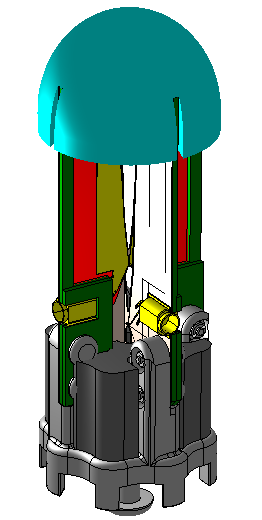
\includegraphics[height=6cm]{Antennas/Vivaldi.png}}
  \centering
  \subfigure[Pattern]{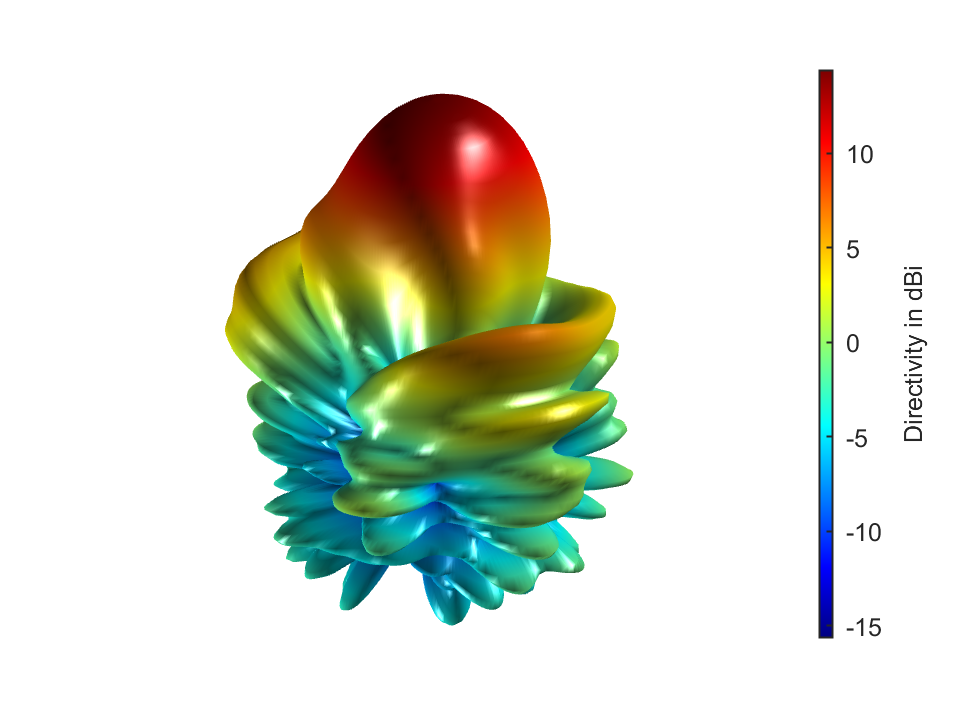
\includegraphics[height=6cm]{Antennas/vivaldi_3D.png}}
\caption{R\&{}S Vivladi TC-TA85CP}
\label{fig:vivpro}
\end{figure}

To show the effects of the different field region high gain/aperture antennas are used as \ac{DUT}; as probe also low gain antennas are used. \ac{DUT} antennas:

\begin{itemize}
\item $\SI{20}{\decibel}$ \ac{SGH} LB-28-20 by A-Info depicted in figure \ref{fig:hornpro}.
\item Array of 2x2 $\SI{20}{\decibel}$ \acp{SGH} with $\SI{27}{\decibeli}$ directivity; the pattern is depicted in figure \ref{fig:othera} (b).
\item 10x1 Patch Array from \cite{7481205}, depicted in figure \ref{fig:10x1a} with $\SI{16}{\decibeli}$ directivity
\end{itemize}

Probe antennas:

\begin{itemize}
\item Hertz dipole with $\SI{1.76}{\decibeli}$ Directivity; Pattern in figure \ref{fig:othera} (d).
\item $\sfrac{\lambda}{2}$-dipole with $\SI{2.15}{\decibeli}$ Directivity; Pattern in figure \ref{fig:othera} (c).
\item R\&{}S experimental patch antenna with $\SI{4}{\decibeli}$ directivity depicted in figure \ref{fig:patchpro}.
\item \ac{OEWG} with $\SI{6}{\decibeli}$ directivity depicted in figure \ref{fig:oewgpro}.
\item \ac{RS} Vivladi TC-TA85CP with $\SI{14}{\decibeli}$ directivity depicted in figure \ref{fig:vivpro}.
\item $\SI{20}{\decibel}$ \ac{SGH} LB-28-20 by A-Info depicted in figure \ref{fig:hornpro}.
\item $\SI{26}{\decibel}$ horn depicted in figure \ref{fig:othera} (a).
\end{itemize}

All physical existing antennas are depicted with there simulation model on the left (a) and their directivity pattern on the right (b). Other impractical antennas such as the $\SI{26}{\decibel}$ horn, simulated by a big waveguide port, the 2x2 $\SI{20}{\decibel}$ \ac{SGH} array, the $\sfrac{\lambda}{2}$-dipole, which is at \ac{mmW} wavelength not realisable, and the Hertz-dipole are only depicted with there pattern in \ref{fig:othera}.\\
The \ac{RS} Vivladi TC-TA85CP is the standard probe antenna at \ac{RS} with a frequency range from $\SI{4}{\giga\hertz}$ to $\SI{87}{\giga\hertz}$, a gain between $\SI{10}{\decibel}$ and $\SI{20}{\decibel}$ and especially the possibility of measuring both polarisations at the same time with a cross-polarization rejection of greater $\SI{20}{\decibel}$. (figure \ref{fig:vivpro})\\
The $\SI{20}{\decibel}$ \ac{SGH} LB-28-20 by A-Info is normally used to calibrate the measurement setup. It is well known with a lot of empirical data. The underlying WR28-waveguide allows a frequency range from $\SI{26.5}{\giga\hertz}$ to $\SI{40}{\giga\hertz}$. A patch antenna is currently in development at \ac{RS}, it is also used for this simulation and measurement but because it is currently not published no further details will be given in this document, except that it has a directivity of $\SI{5}{\decibeli}$, a realized gain of $\SI{3.5}{\decibel}$ and the pattern depicted in figure \ref{fig:patchpro}. 

\subsection{Result}

The simulation results for all three tested \acp{DUT} is plotted in figure \ref{fig:simres}. In (a), (c) and (e) the \ac{TMP} is plotted over the measurement distance and in (b), (d) and (f) the \ac{EIRP} in the main lobe of the \ac{DUT} is plotted over the measurement distance. The tendency is that, at the same distance the \ac{TMP} error of low directivity probes, such as dipole, patch and \ac{OEWG} is lower than the \ac{TMP} error of high directivity probes, such as Vivaldi and \ac{SGH}. Some similarities between the \ac{TMP} measurement of the \ac{SGH} and the patch array can be found in the course of the graphs. Concluding the \ac{TMP} error is with low directivity probing always lower then $\SI{0.5}{\decibel}$ for greater distances as Derat distance. The individual graph, as well as for the \ac{TMP} and for the \ac{EIRP} in the main lobe, is dependent of the combination of \ac{DUT} and probe. The coarse graph shape of the probe less simulation from figure \ref{fig:beamcpmp} (c) is recognisable in this complete simulation in \ref{fig:simres}. \todo{schreib hier noch mehr}

\begin{figure}[H]
  \centering
  \subfigure[TMP; DUT: $\SI{20}{\decibel}$ SGH]{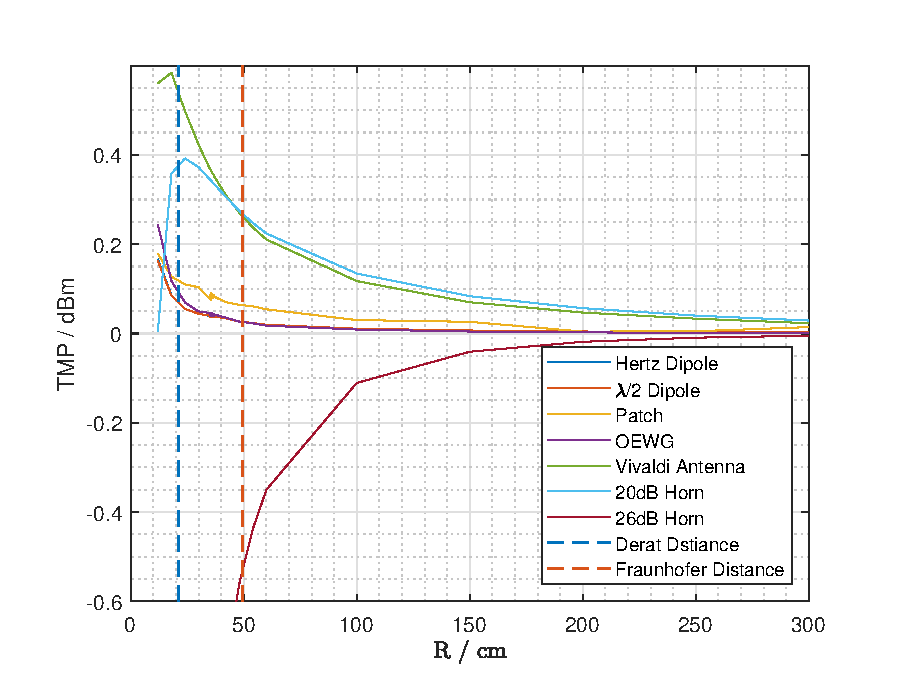
\includegraphics[width=0.49\textwidth]{Matlab/trpDistVivTMP.eps}}
  \centering
  \subfigure[Main EIRP; DUT: $\SI{20}{\decibel}$ SGH]{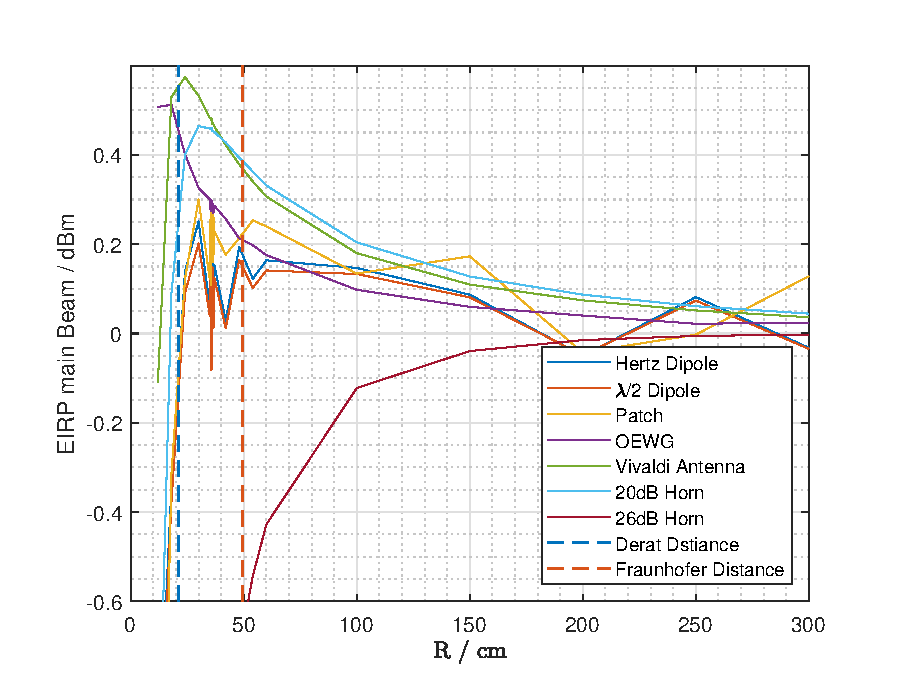
\includegraphics[width=0.49\textwidth]{{Matlab/trpDistVivEIRP.eps}}}
  \centering
  \subfigure[TMP; DUT: 10x1 patch array \cite{7481205}]{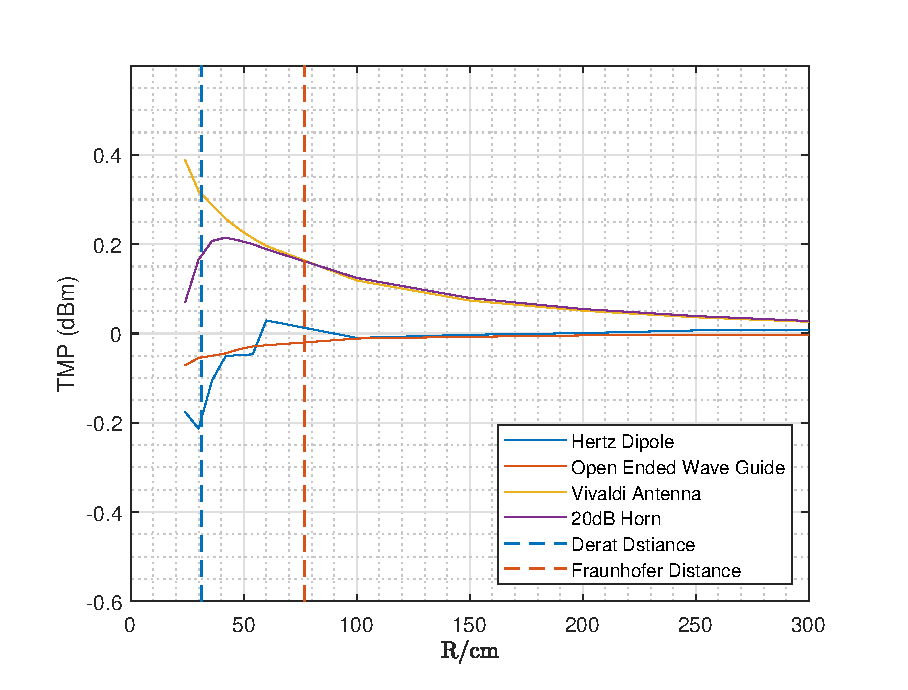
\includegraphics[width=0.49\textwidth]{Matlab/trpDistPaATMP.eps}}
  \centering
  \subfigure[Main EIRP; DUT: 10x1 patch array \cite{7481205}]{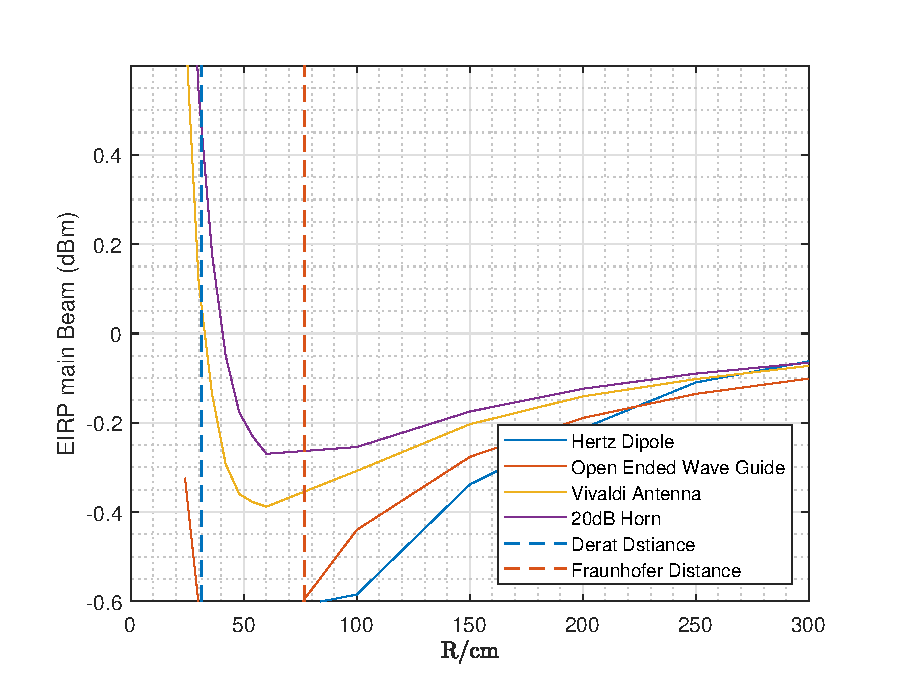
\includegraphics[width=0.49\textwidth]{{Matlab/trpDistPaAEIRP.eps}}}
  \centering
  \subfigure[TMP; 2x2 $\SI{20}{\decibel}$ SGH Array]{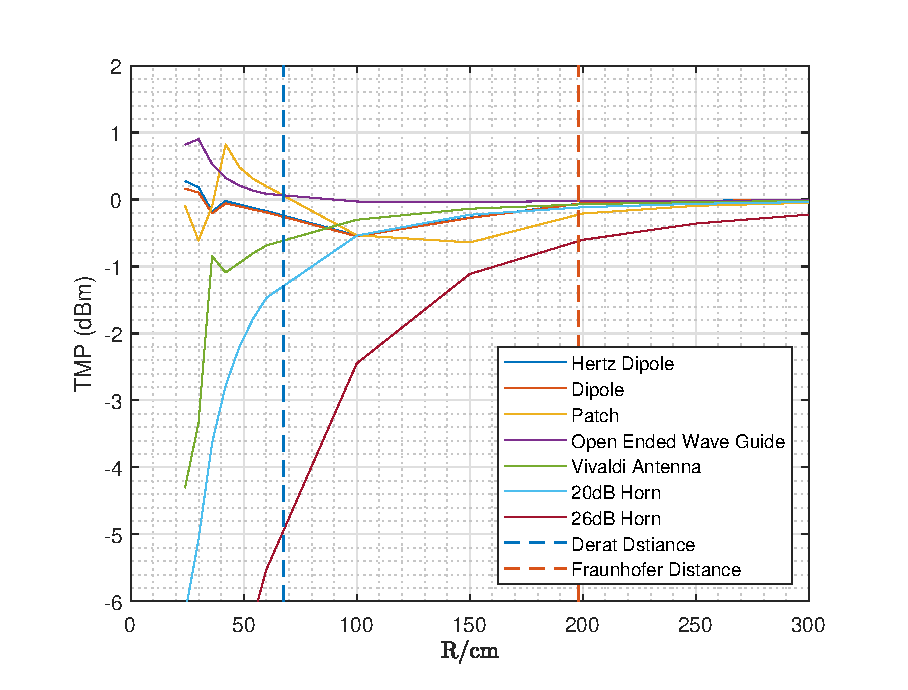
\includegraphics[width=0.49\textwidth]{Matlab/trpDistH2TMP.eps}}
  \centering
  \subfigure[Main EIRP; 2x2 $\SI{20}{\decibel}$ SGH Array]{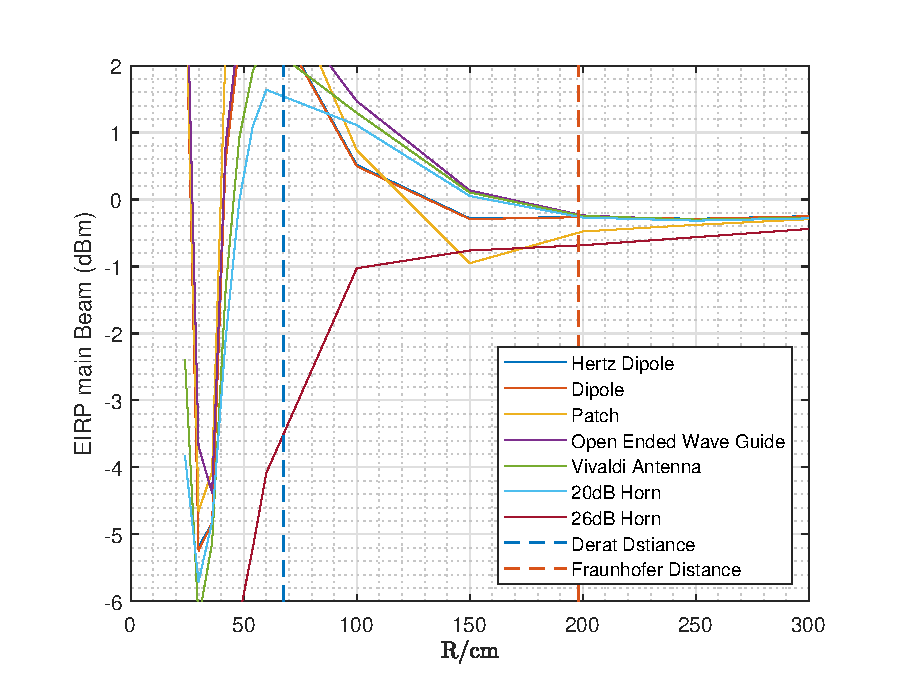
\includegraphics[width=0.49\textwidth]{{Matlab/trpDistH2EIRP.eps}}}
\caption{Simulation results}
\label{fig:simres}
\end{figure}

\section{Measurement}

\begin{figure}[H]
\centering
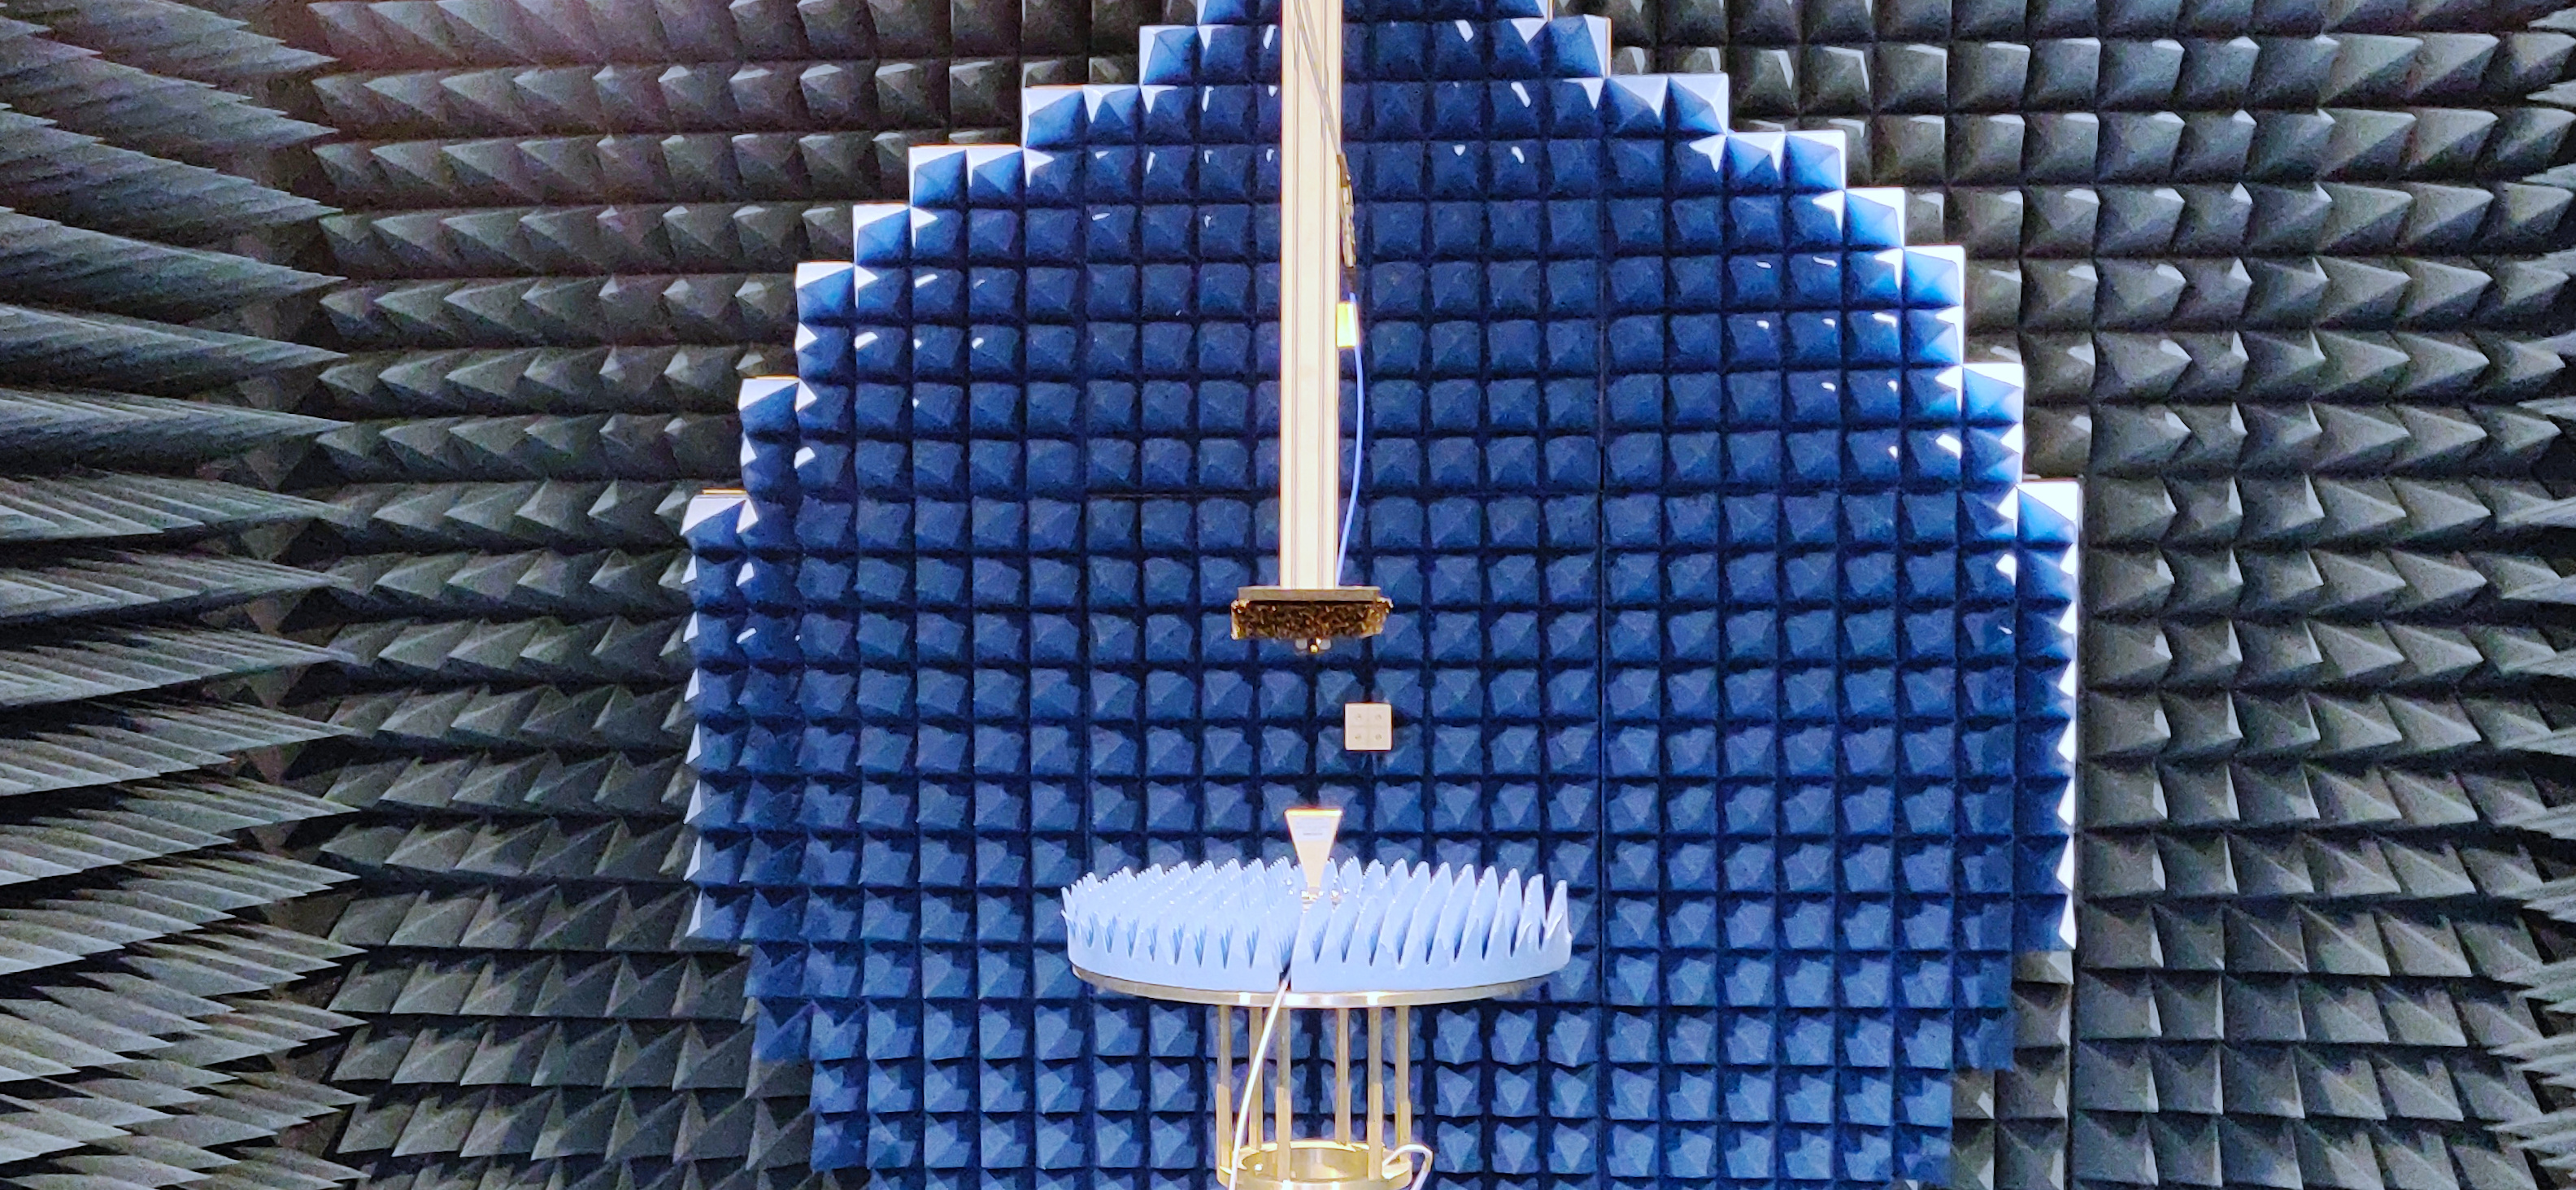
\includegraphics[width=0.8\textwidth]{big-chamber.jpeg}
\caption{OTA Measurement for minimum rangelength measurement series; DUT: $\SI{20}{\decibel}$ SGH; probe: Patch}
\label{fig:otameas}
\end{figure}

To proof the introduced simulation to investigating \ac{NF} probing for \ac{TRP} measurements this test is done in a \ac{WPTC} depicted in figure \ref{fig:otameas}, located in the \ac{RS} headquarters in Munich using a \ac{RS} \ac{VNA} 67.

\subsection{Implementation}

 Because of the high cable loss resulting from long cables caused by the big chamber a $\SI{40}{\decibel}$ azimuth amplifier is used. Only the A-Info $\SI{20}{\decibel}$ \ac{SGH} was used as \ac{DUT} on the azimuth table with it's aperture in the center of rotation. This adds an other $\SI{3}{\centi\meter}$ radius to the phase center. Occupying a low gain probe such as the Patch, the maximum range length of about $\SI{1.1}{\meter}$ and a \ac{RBW} of $\SI{100}{\hertz}$ results in a dynamic range of about $\SI{20}{\decibel}$. This is not pleasant to plot the pattern, but it's sufficient to compute an adequate \ac{TMP}. To adjust the radius a aluminium profile is used refer to figure \ref{fig:otameas}. Because of the mounting at azimuth the elevation can only be measured from $\theta_\text{min}=\SI{0}{\degree}$ and $\theta_\text{max}=\SI{85}{\degree}$ which is sufficient regarding the \ac{SGH}s pattern in figure \ref{fig:hornpro}. As in the simulation a $\SI{5}{\degree}$-\ac{CSSG} is used with swept azimuth and therefore hardware triggering from the positioner to the \ac{VNA}. So that one \ac{TRP} measurement takes around $\SI{2}{\min}$.

\subsection{Set Up}

\begin{figure}[H]
  \centering
  \subfigure[WR28 OEWG 1]{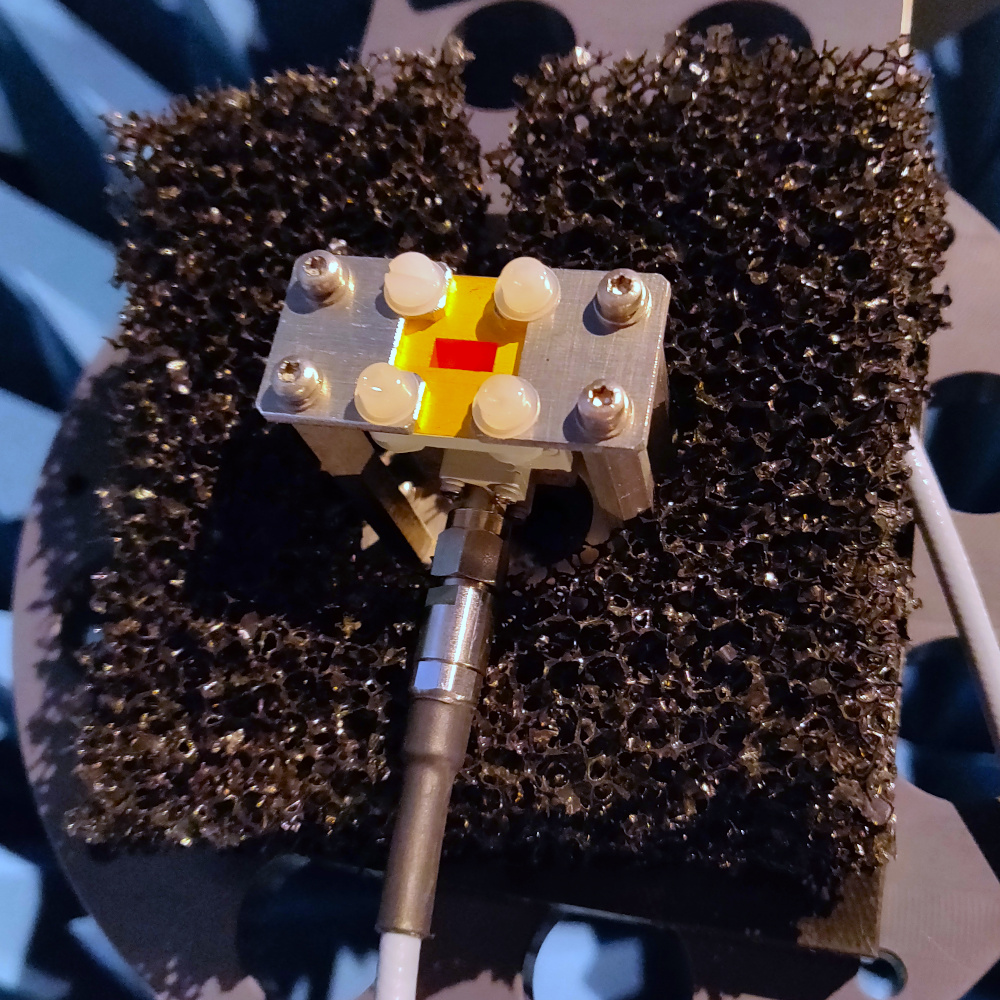
\includegraphics[width=0.3\textwidth]{OEWG-Imp1.jpg}}
  \centering
  \subfigure[WR28 OEWG 2]{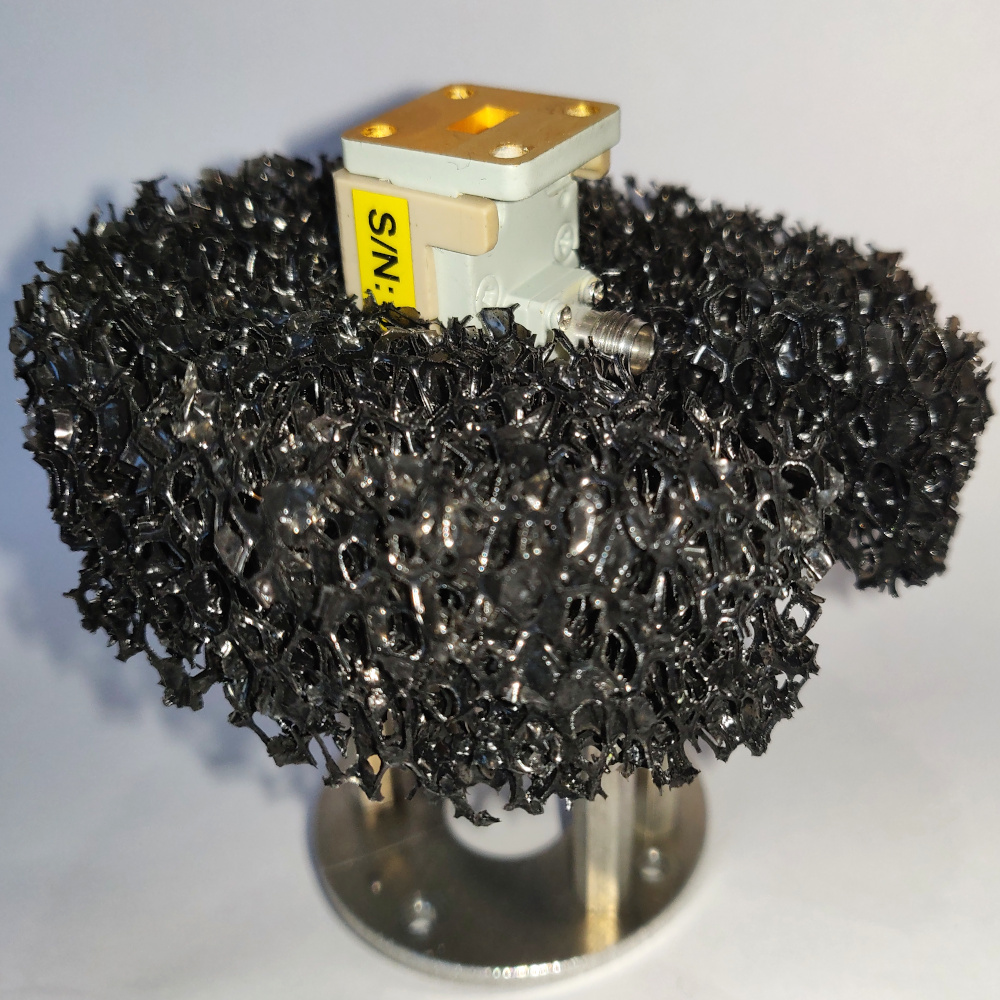
\includegraphics[width=0.3\textwidth]{OEWG.jpg}}
  \centering
  \subfigure[Mounted Patch antenna]{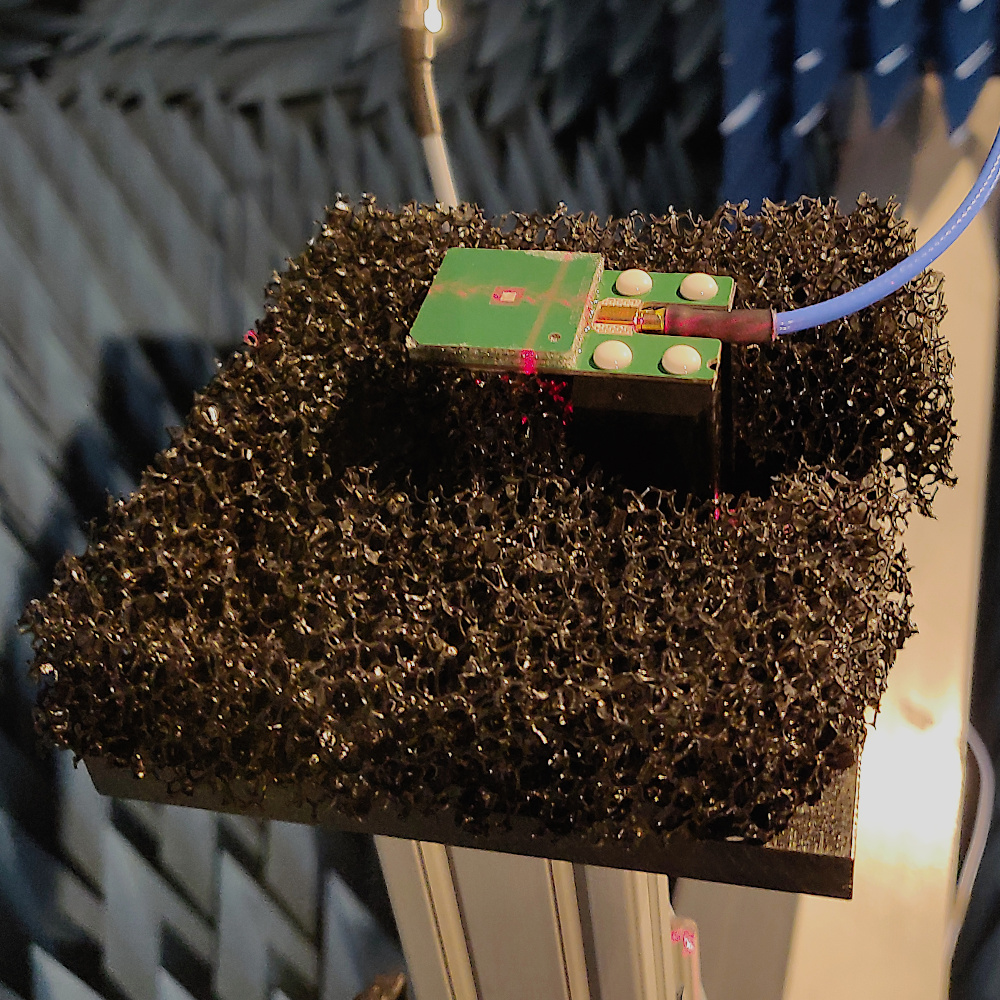
\includegraphics[width=0.3\textwidth]{Patch.jpg}}
\caption{Real implementation of probe antennas}
\label{fig:realprobe}
\end{figure}

The minimum and maximal measurement sphere radius varies because of the probe mounting from around $\SI{10}{\centi\meter}$ to around $\SI{115}{\centi\meter}$. From $\SI{10}{\centi\meter}$ to $\SI{16}{\centi\meter}$ radius $\SI{1}{\centi\meter}$, from $\SI{16}{\centi\meter}$ to $\SI{20}{\centi\meter}$ $\SI{2}{\centi\meter}$ and than $\SI{5}{\centi\meter}$ radius increment is taken. The measurement is carried out by using the $\SI{20}{\decibel}$ \ac{SGH} LB-28-20 by A-Info (figure \ref{fig:hornpro}), the Vivaldi (figure \ref{fig:vivpro}), the Patch (figure \ref{fig:realprobe} (c)) and the two \ac{OEWG} implementations (figure \ref{fig:realprobe} (a) and (b)) as probe and the $\SI{20}{\decibel}$ \ac{SGH} as \ac{DUT}. There are some issues with the probe implementations depicted in figure \ref{fig:realprobe}:

\begin{enumerate}[label=(\alph*)]
\item Because no WR28 \ac{OEWG} antenna was available, a WR28 wave guide adapter and a \ac{SGH} mounting was first taken. With the metal in front of the aperture the \ac{FF} pattern differs from a real \ac{OEWG} and the directivity increases by around $\SI{4}{\decibel}$. This was simulated in CST\texttrademark nad the resulting antenna pattern is plotted in figure \ref{fig:oewgimpone}.
\item With an other mounting the aperture is free from additional metal. The problem is here, that the metal plate surrounding the opening of the wave guide reflects the \ac{EM} waves emitted to it. This leads to standing waves in the \ac{NF}.
\item The patch is a omnidirectional radiator (refer to figure \ref{fig:patchpro}). With the absorbers, the directivity of this antenna is rising, because the \ac{TRP} is sinking by absorbing the backwards orientated radiation. Additionally the patch antenna is placed on a ground plane, which leads similar to the wave guide adapter from (b) to standing waves.
\end{enumerate}

\subsection{Result}

\begin{figure}[H]
  \centering
  \subfigure[TMP over measurement distance]{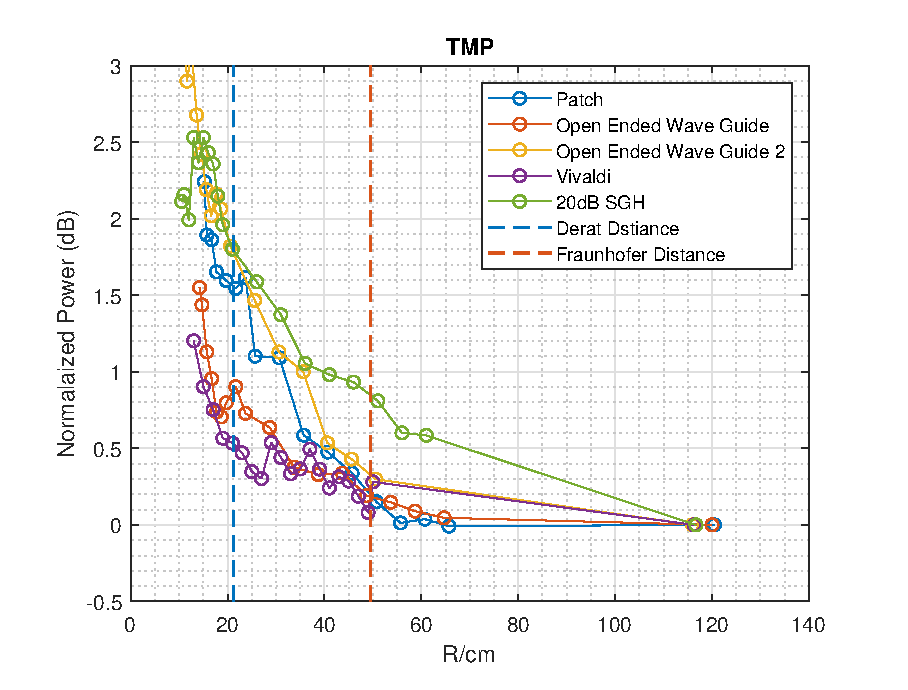
\includegraphics[width=0.49\textwidth]{Matlab/measSGHTMP.eps}}
  \centering
  \subfigure[Main EIRP over measurement distance]{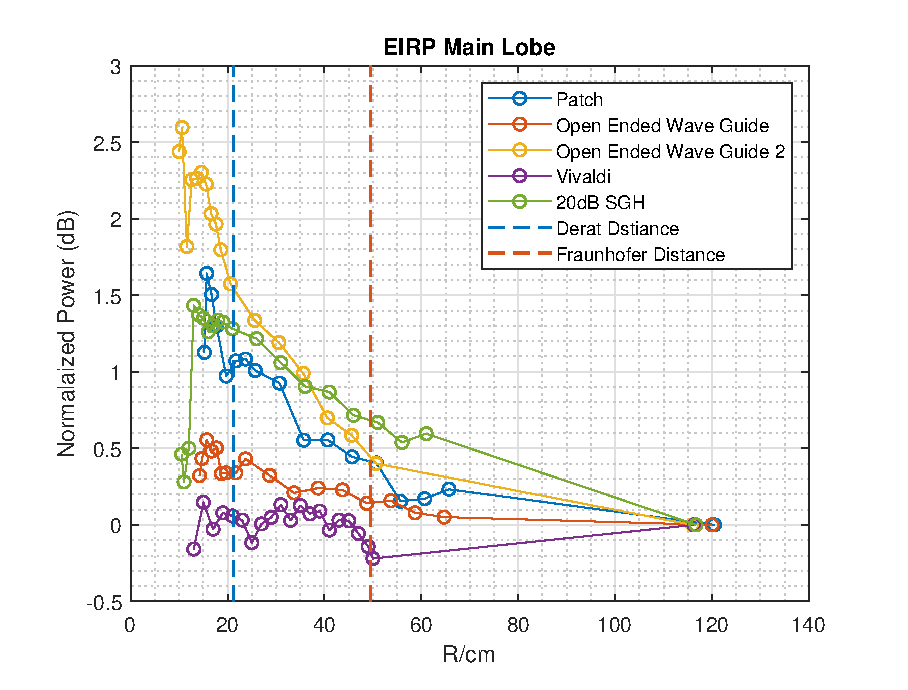
\includegraphics[width=0.49\textwidth]{{Matlab/measSGHEIRP.eps}}}
\caption{Measurement result: DUT $\SI{20}{\decibel}$ SGH}
\label{fig:meastrpdistviv}
\end{figure}

\todo{reformulieren}

As described in the section above there are some issues with both \ac{OEWG} implementations and the patch antenna. That explains the unexpected course of these graphs. The exception would be that the directivity of the probe antennas is positively correlated with the measured \ac{TMP} error. This is seen in figure \ref{fig:meastrpdistviv} (a) between \ac{SGH} and Vivaldi antenna.\\
Direct interaction/coupling between the probe and the \ac{DUT} could not be simulated. This explains the generally higher error level. It has a very big impact on probes with flat metal surfaces tangential to the \ac{DUT}. These metal surfaces lead to standing waves and thereby to a greater measurement result. This effect is mostly seen in figure \ref{fig:meastrpdistviv} (a) by the second \ac{OEWG} implementation and the patch, which have less error in \ac{FF} while the curves sharply rise at Fraunhofer distance.\\
Viewing the \ac{EIRP} in the main lobe, this phenomena is also recognisable. Also the shape of the curve of the \ac{SGH} is similar to the simulation. A real statement must be made in the future by using a real \ac{OEWG} probe without any tangential area and repeat the measurement. The patch antenna would need to be redesigned for \ac{NF} probing. A simpler solution could be to design a new mount for the patch antenna with a small angle offset to scatter the mirrored wave away from the \ac{DUT}.





